\section{Anwendungsfaelle}
\begin{figure}[H]
    \centering
    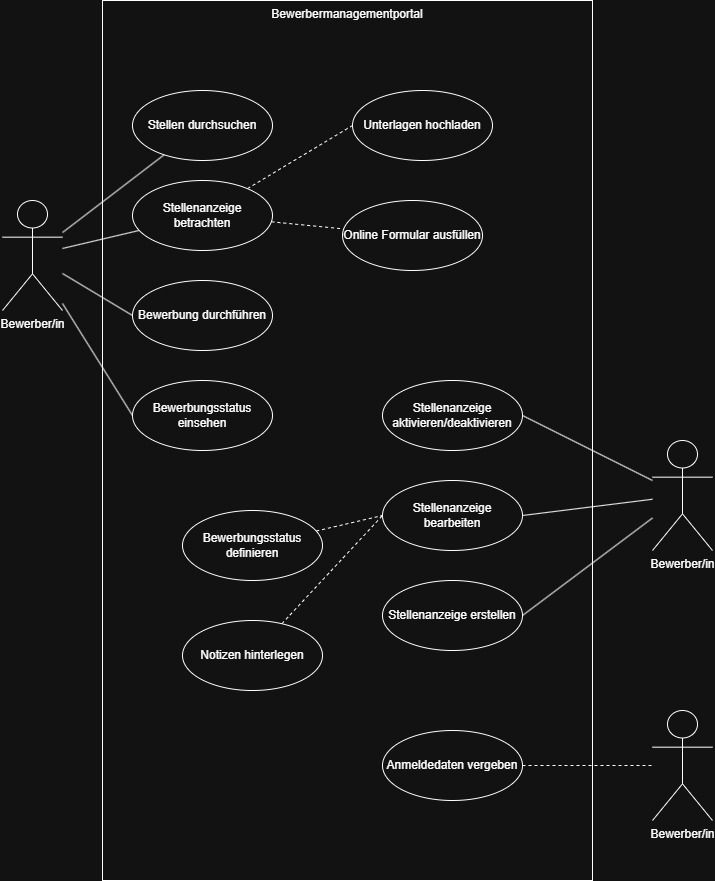
\includegraphics[width=0.7\textwidth]{UseCase.jpg}
    \caption{Anwendungsfaelle mittels UseCase-Diagramm abgebildet.}
    \label{fig:useCase}
\end{figure}

\section{Wireframes und Mockups des UI}
\begin{figure}[H]
    \centering
    
\includegraphics[width=0.7\textwidth]{LandingPage.png}
    \caption{Mockup der Landing Page.}
    \label{fig:landingPage}
\end{figure}
\begin{figure}[H]
    \centering
    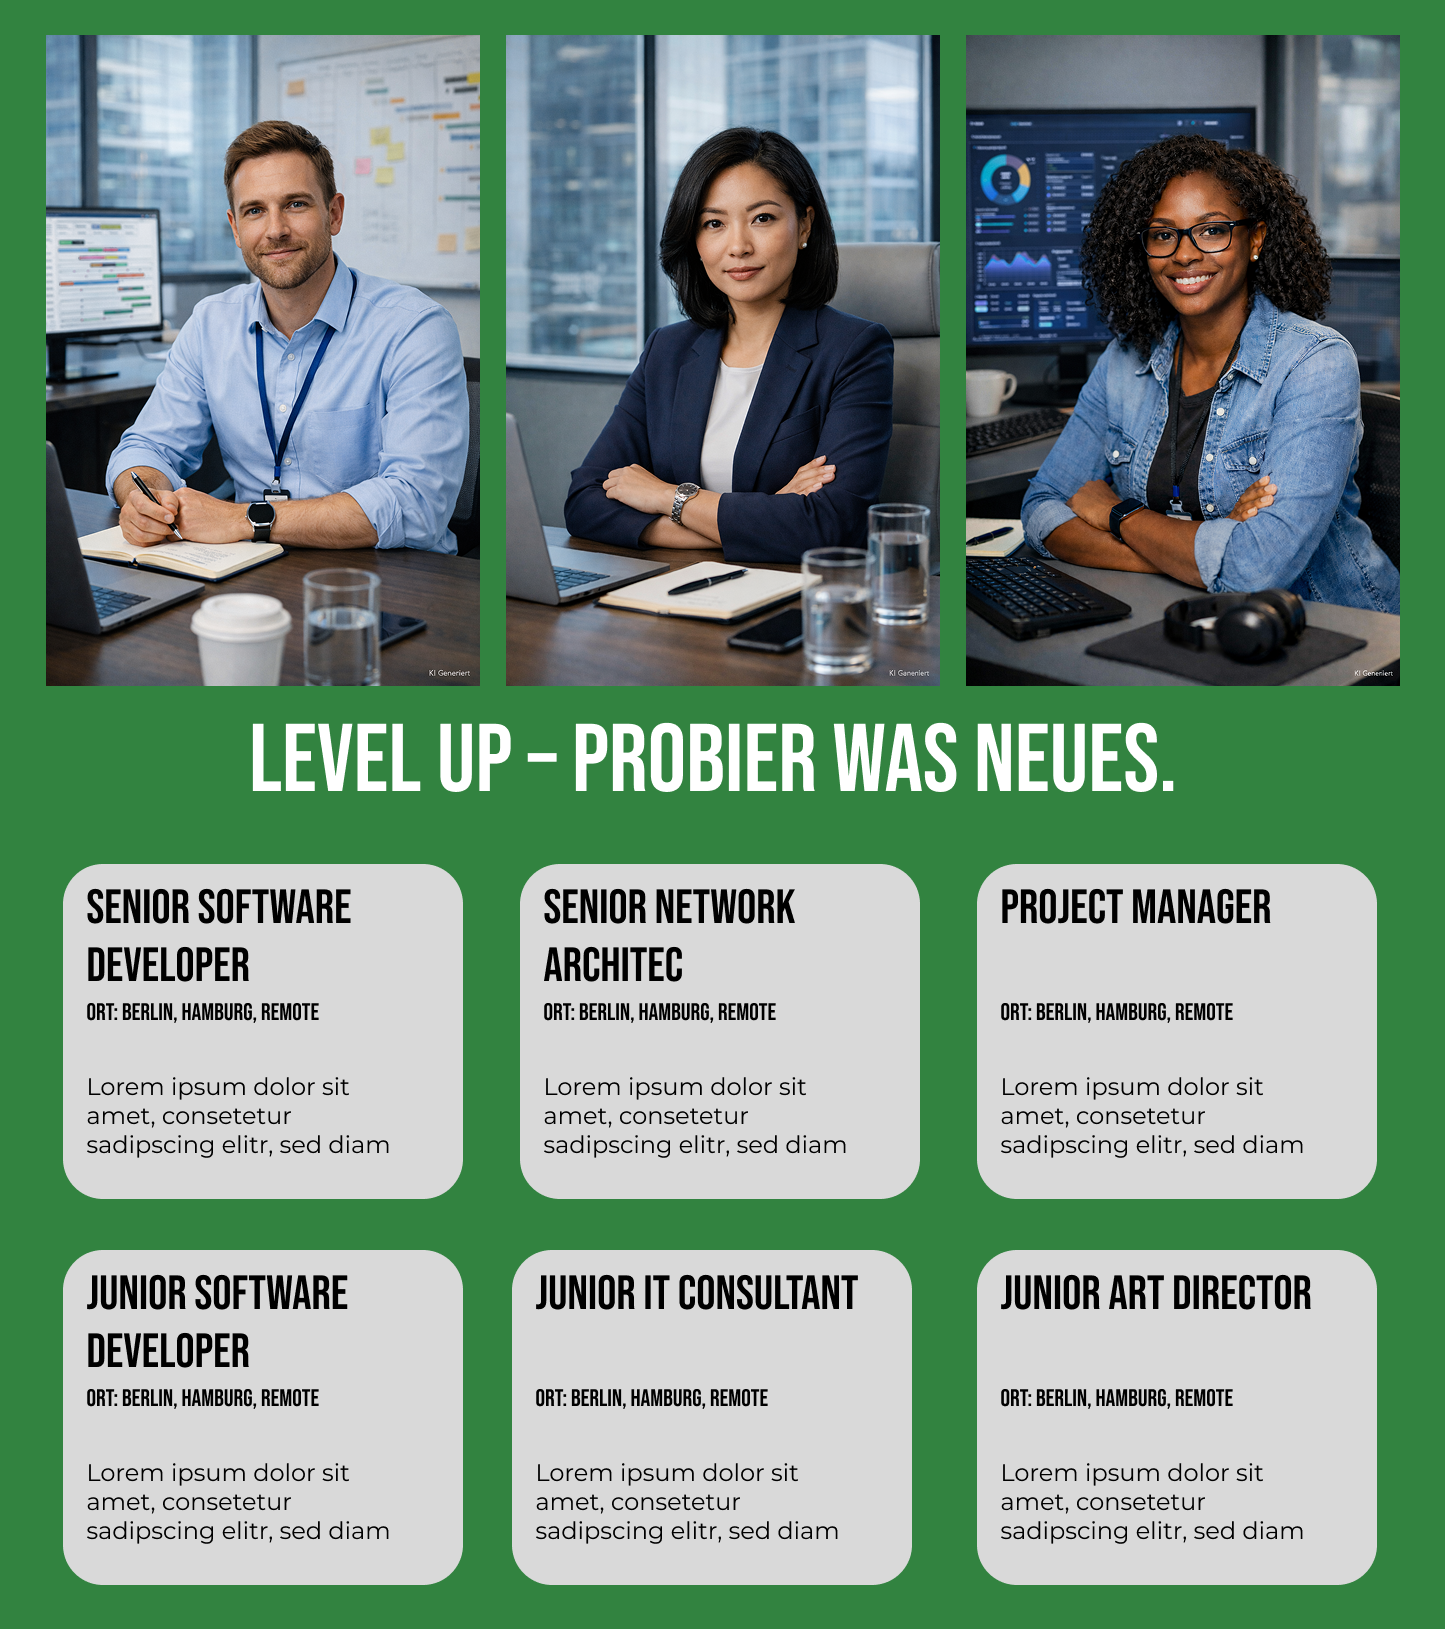
\includegraphics[width=0.7\textwidth]{StellenOverview.png}
    \caption{Mockup der Stellenübersicht.}
    \label{fig:stellenOverview}
\end{figure}
\begin{figure}[H]
    \centering
    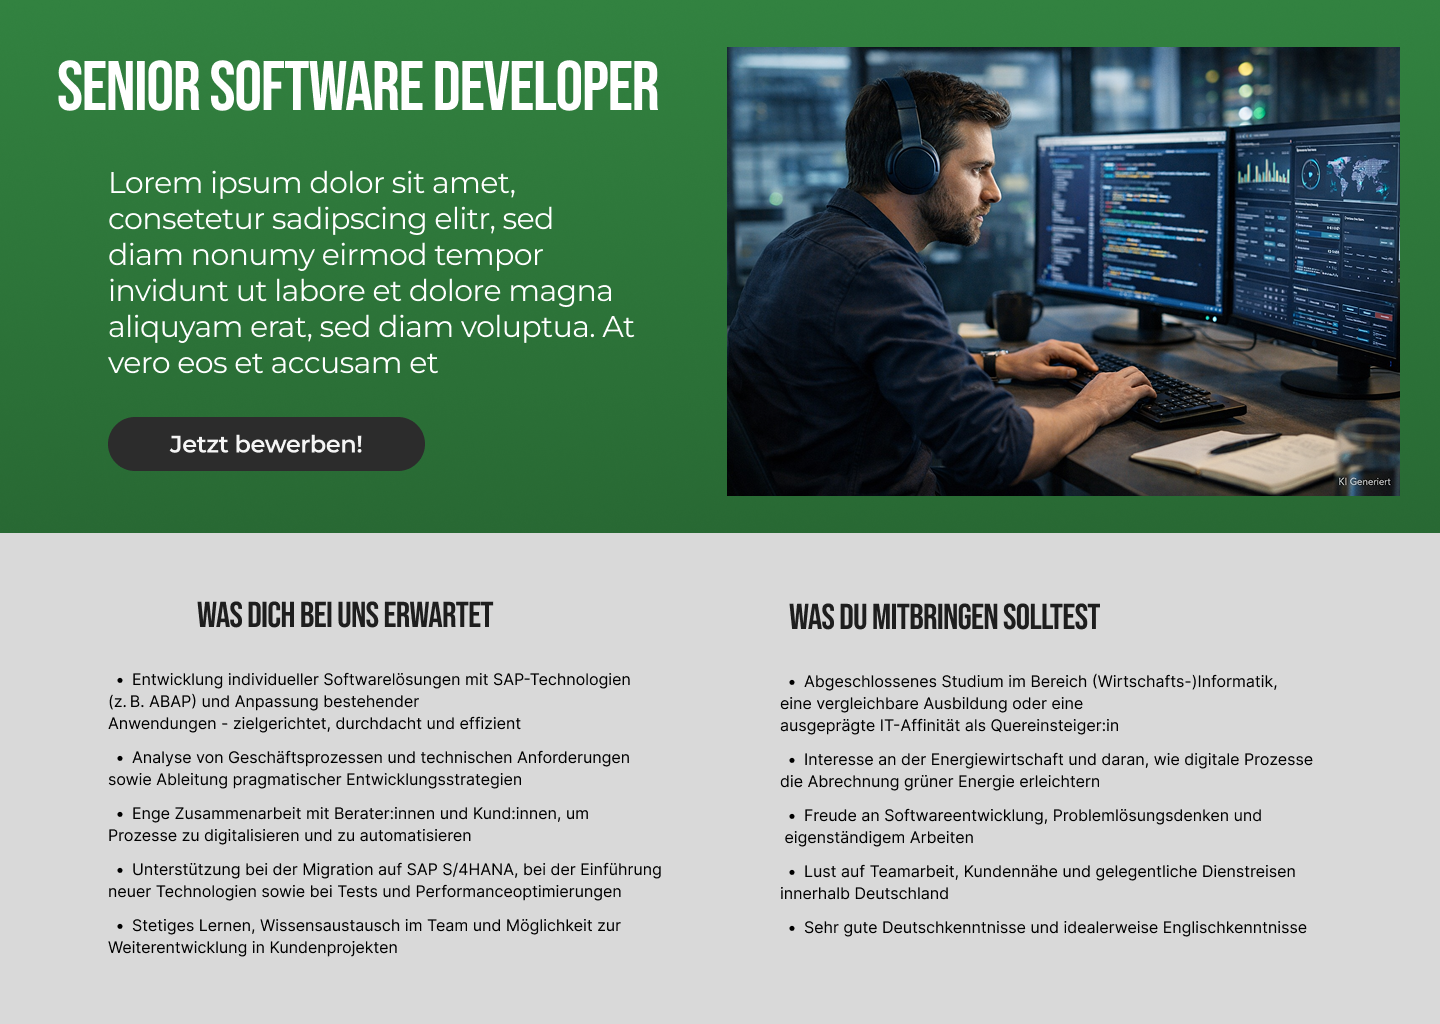
\includegraphics[width=0.7\textwidth]{Stellenanzeige.png}
    \caption{Mockup der Stellendetailseite.}
    \label{fig:stelle}
\end{figure}
\begin{figure}[H]
    \centering
    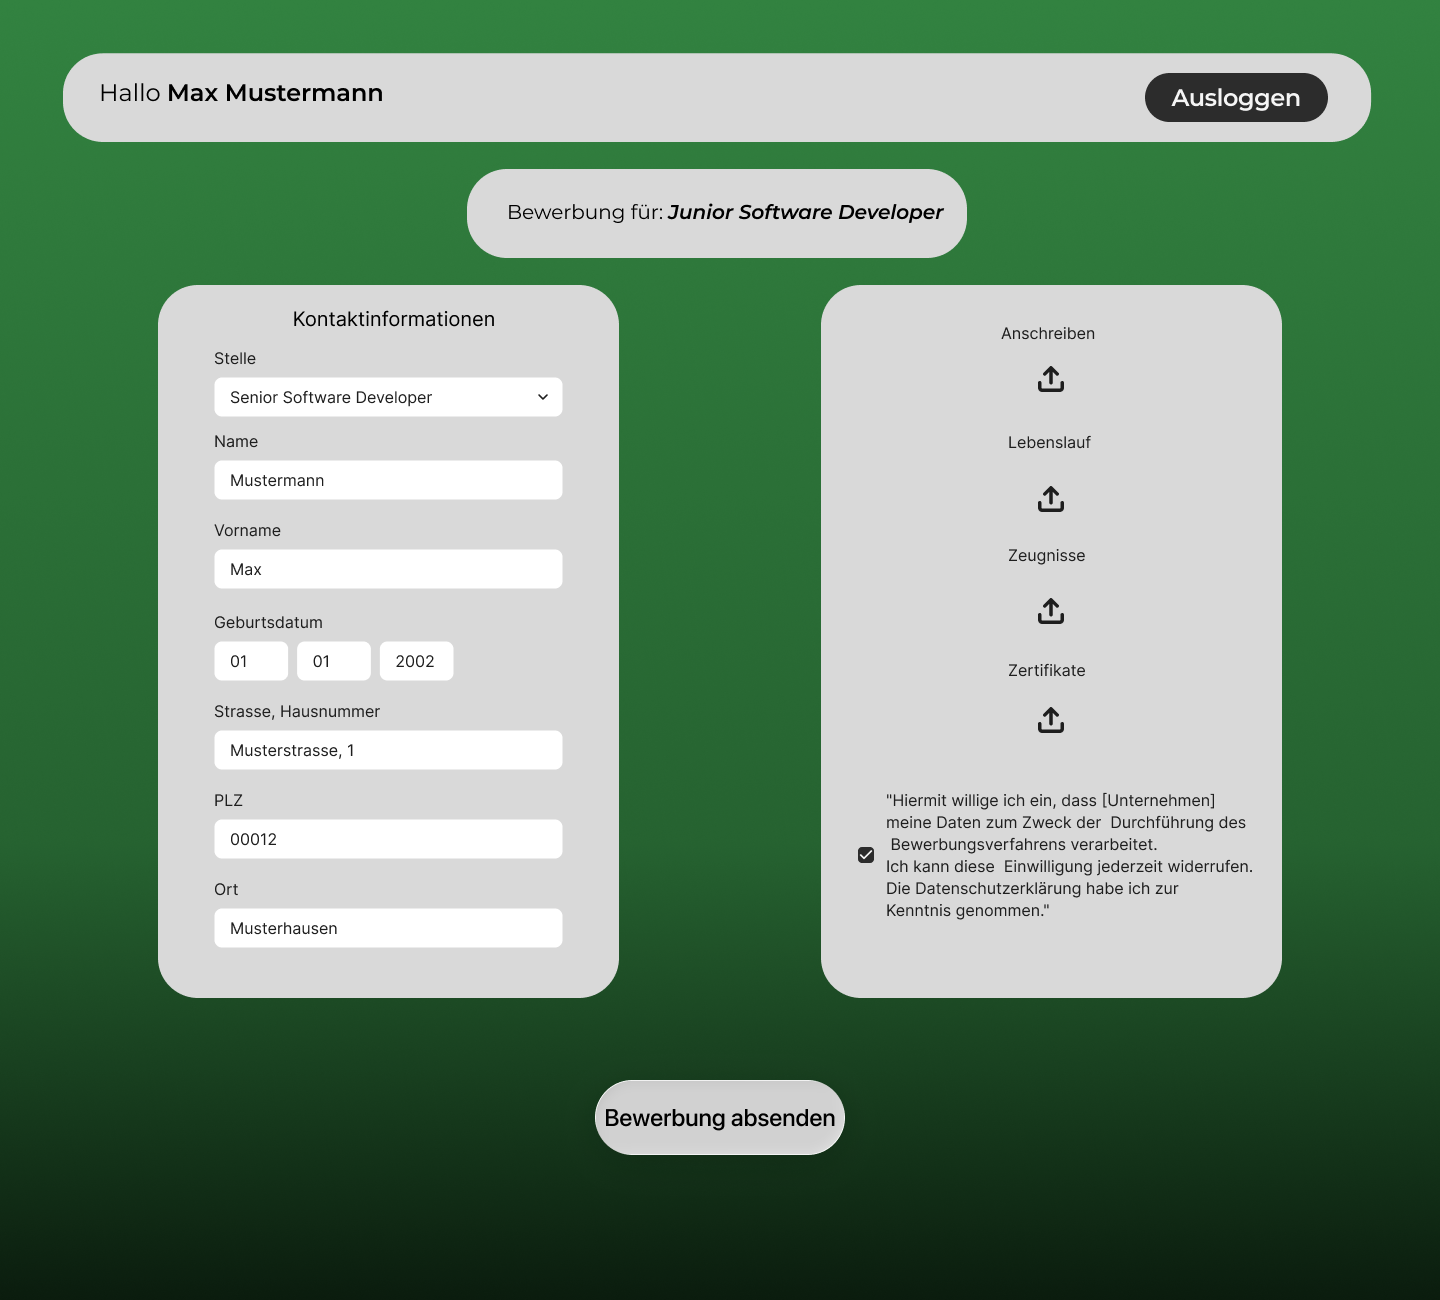
\includegraphics[width=0.7\textwidth]{Bewerbungsformular.png}
    \caption{Wireframe des Bewerbungsformulars.}
    \label{fig:bewerbungFormular}
\end{figure}
\begin{figure}[H]
    \centering
    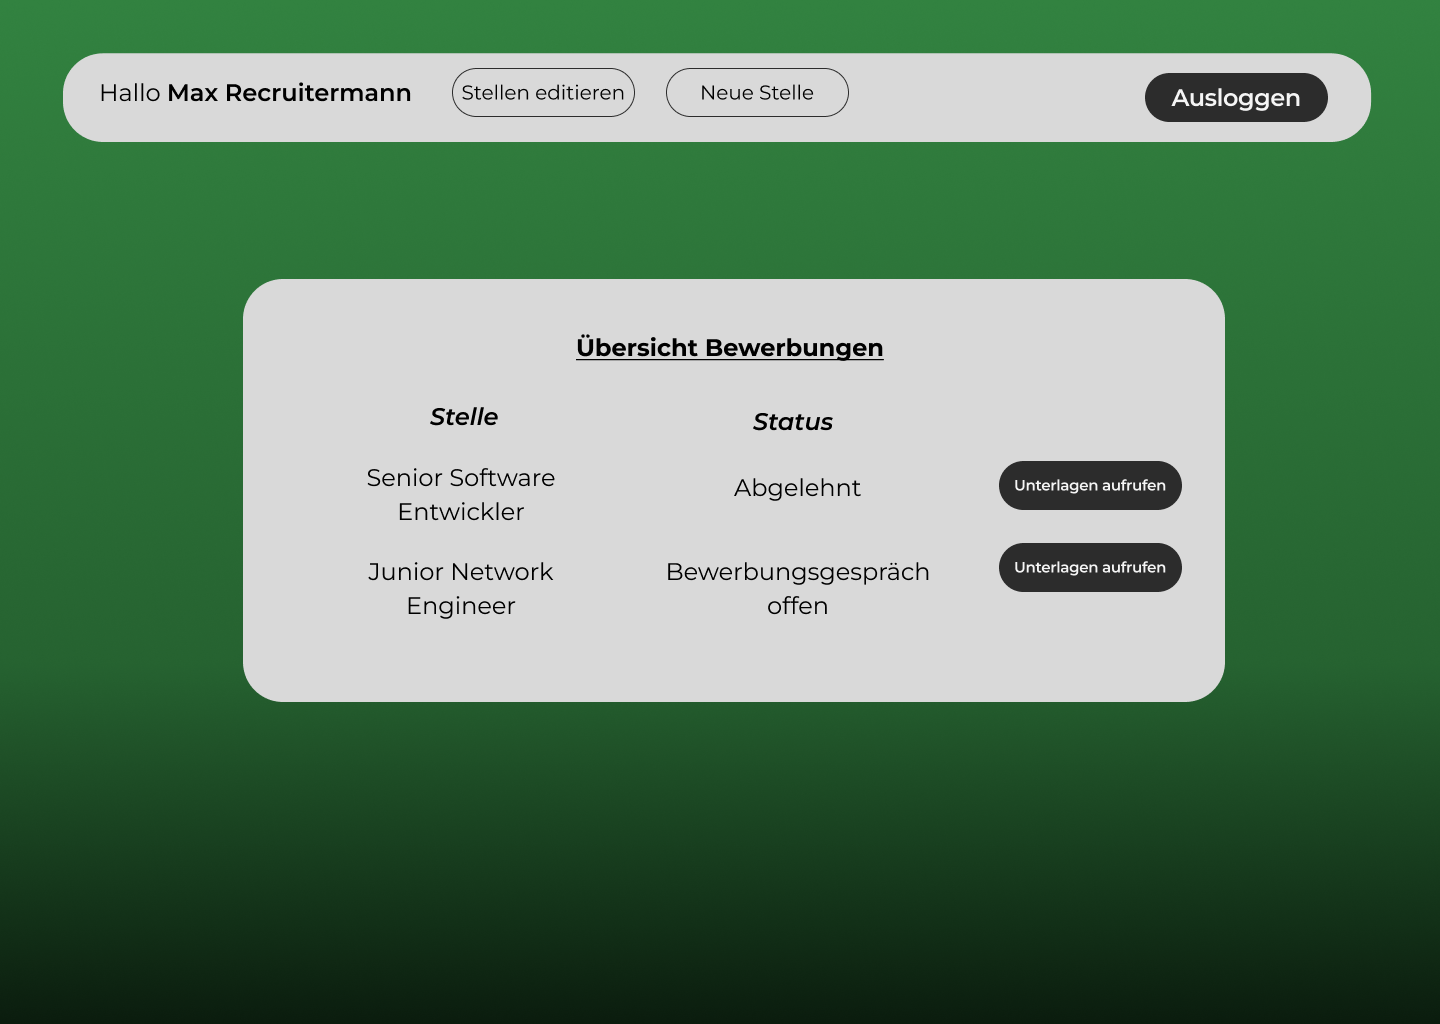
\includegraphics[width=0.7\textwidth]{RecruiterDashboard.png}
    \caption{Wireframe des Recruiter-Dashboards.}
    \label{fig:recruiterDashboard}
\end{figure}

\section{Datenmodell}

\section{Vergleich moeglicher Technologien}

\section{Vergleich moeglicher Technologien}


\begin{table}[htbp]
\centering
\small
\begin{tabularx}{\textwidth}{lXXX}
\toprule
Kriterium & PHP & Node.js & Spring Boot \\
\midrule
Einstieg und Lernaufwand
& Sehr gering
& Mittel, Kenntnisse in JavaScript und zugehörigen Frameworks erforderlich
& Hoch, Kenntnisse in Java und Framework-Konfiguration nötig \\

Entwicklungsaufwand
& Schnell umsetzbar für klassische Webanwendungen
& Flexibel, aber oft zusätzliche Frameworks nötig
& Strukturierte Entwicklung, aber relativ komplex \\

Infrastruktur
& Läuft direkt auf klassischen Webservern
& Benötigt Node.js-Runtime
& Benötigt Java-Runtime \\

Projektkomplexität
& Gering bis mittel
& Gute Skalierbarkeit für moderne Webanwendungen
& Für große Enterprise-Anwendungen geeignet \\

Entwicklungszeit für MVP
& Kurz
& Mittel
& Eher länger \\

Eignung für dieses Projekt
& Sehr gut geeignet
& Okay, aber höherer Setup-Aufwand nötig
& Für den Projektumfang überdimensioniert \\
\bottomrule
\end{tabularx}
\caption{Ergebnisse des Tech-Stack-Vergleichs}
\label{tab:vglBackend}
\end{table}

\begin{table}[htbp]
\centering
\small
\begin{tabularx}{\textwidth}{lXXX}
\toprule
Kriterium & SQLite & MySQL & PostgreSQL \\
\midrule
Installation
& Keine separate Installation erforderlich
& Datenbankserver muss installiert werden
& Datenbankserver muss installiert werden \\

Systemarchitektur
& Embedded-Datenbank (dateibasiert)
& Client-Server-Datenbanksystem
& Client-Server-Datenbanksystem \\

Administrationsaufwand
& Sehr gering
& Mittel
& Mittel bis höher \\

Skalierbarkeit
& Für kleine Anwendungen geeignet
& Gut skalierbar
& Sehr gut skalierbar \\

Mehrbenutzerbetrieb
& Eingeschränkt
& Sehr gut geeignet
& Sehr gut geeignet \\

Einsatzgebiet
& Prototypen, kleine Anwendungen
& Webanwendungen und CMS-Systeme
& Komplexe Anwendungen und große Systeme \\

Geeignet für dieses Projekt
& Sehr gut geeignet
& Möglich, aber mehr Infrastruktur nötig
& Für Projektumfang nicht erforderlich \\
\bottomrule
\end{tabularx}
\caption{Vergleich verschiedener Datenbanksysteme}
\label{tab:dbvergleich}
\end{table}


\section{Architekturbild}
\begin{figure}[H]
    \centering
    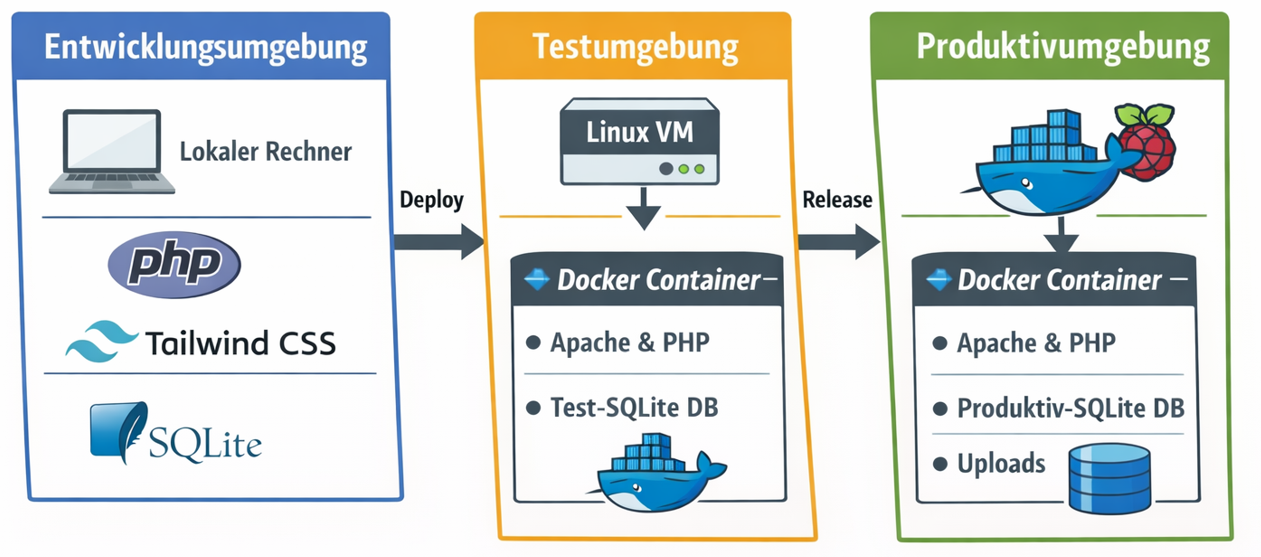
\includegraphics[width=0.8\textwidth]{archBild.png}
    \caption{Architekturbild.}
    \label{fig:archBild}
\end{figure}
